%%January 20- 2002
%\documentclass[wrr]{agu2001}
\documentclass{report}


\usepackage{natbibDK}
\usepackage{amsmath}
\usepackage{amssymb}
\usepackage[dvips]{graphicx}


\usepackage[T1]{fontenc}        %for danish letters
\usepackage[latin1]{inputenc}   %for danish letters




\begin{document}

%% ------------------------------------------------------------------------ %%
%
%  TITLE
%
%% ------------------------------------------------------------------------ %%


\title{Formler til Milj\ostyrrelsen}

%% ------------------------------------------------------------------------ %%
%
%  AUTHORS AND AFFILIATIONS
%
%% ------------------------------------------------------------------------ %%

\author{Mikkel Mollerup}




\chapter{Water movement}


\section{Richard's Equation}

The water flow in porous media can be described with the formula of
Richard. The equation is derived here. The water flux density
vector, $\mathbf{q}$ can be calculated by the Darcy�s law. For a
two-dimensional vertical transect it yields:
\begin{equation}
\mathbf{q}=-\mathbf{K}(\psi)\nabla(\psi + z) \label{eq:darcy}
\end{equation}
where $\mathbf{K}(\psi)$ is the hydraulic conductivity tensor,
$\psi$ is the potential head. The x-axis is chosen in horizontal
direction and the z-axis is positive upwards. The conductivity
tensor can be expressed as:
\begin{equation}
\mathbf{K}=\begin{bmatrix} K_{xx} & K_{xz} \\ K_{zx} & K_{zz}
 \end{bmatrix}
\end{equation}
For a model with rectangular cells we have chosen that the
 principal directions of the anisotropic medium are parallel to
 the $x$- and $z$-axis, i.e.
\begin{equation}
\mathbf{K}=\begin{bmatrix} K_{xx} & 0 \\ 0 & K_{zz}
 \end{bmatrix}
\end{equation}
The mass balance for the system gives
\begin{equation}
\frac{\partial \theta}{\partial t}=-\nabla \cdot \mathbf{q}
-\Gamma \label{eq:continuity}
\end{equation}
where $\theta$ is the volumetric water content and $\Gamma$ is the
sink term. The partial differential equation can be developed by
combining Darcy�s law, equation \ref{eq:darcy} and the mass balance,
equation \ref{eq:continuity}, thus
\begin{equation}
\frac{\partial \theta}{\partial t}=\nabla \cdot
\left(\mathbf{K}(\psi)\nabla (\psi + z)\right) - \Gamma
\label{eq:richards}
\end{equation}
This is known as Richard's equation. For the modeling is assumed
that the soil-water retention is without hysteresis, i.e. there is a
unique relation between the matrix pressure potential and the water
content.

To solve Richard's equation it is necessary to specify initial and
boundary conditions. The boundary conditions specify a combination
of $\psi$ and its derivative on the boundary. Furthermore it is
possible to use different forms of flux (Neumann) and predescribed
pressure (Dirichlet) boundary conditions. The problem to be solved
for determining the water movement can be summarized to
%%% with moustages %%%
\begin{equation}
\begin{cases}
\frac{\partial \theta}{\partial t}=\nabla \cdot
\left(\mathbf{K}(\psi)\nabla (\psi + z) \right)-\Gamma & \text{in}\  \Omega \\
\mathbf{\bar{n}} \cdot \left(\mathbf{K}(\psi)\nabla (\psi + z)
\right)=
-q & \text{on}\ \partial \Omega^{N} \\
\psi=\psi_0 & \text{on}\ \partial \Omega^{D}
\end{cases}
\label{eq:watermovement}
\end{equation}
%%%%%%%%%%%%%%%%%%%%%%%
%%% without moustages %%%
%\begin{eqnarray}
%&& \frac{\partial \theta}{\partial t}=\nabla \cdot
%\left(\mathbf{K}(\psi)\nabla (\psi + z) \right)-\Gamma \ \text{in}\  \Omega  \nonumber \\
%&&\mathbf{\bar{n}} \cdot \left(\mathbf{K}(\psi)\nabla (\psi + z)
%\right)=
%-q \ \text{on}\ \partial \Omega^{N} \nonumber \\
%&&\psi=\psi_0 \ \text{on}\ \partial \Omega^{D}
%\label{eq:watermovement}
%\end{eqnarray}
%%%%%%%%%%%%%%%%%%%%%%%%%%
where $\mathbf{\bar{n}}$ is the outward unit normal, and $q$ is the
magnitude of the outward flow from the domain. $\psi_0$ is the
predescribed pressure at the boundary. $\Omega$ is the soil domain.
$\partial\Omega^{N}$ and $\partial\Omega^{D}$ are part of the
boundary of $\Omega$ with Neumann and Dirichlet boundaries,
respectively such that $\partial\Omega=\partial\Omega^{N} \cup
\partial\Omega^{D}$. Each of $\partial\Omega^{N}$ and
$\partial\Omega^{D}$ are not necessarily one continuous curve piece.
A special case of the Neumann boundary conditions is often applied
for the lower boundary condition, viz. it is assumed that the flow
it is only driven by gravity (gravity boundary condition), i.e.
$\partial \psi/
\partial x= \partial \psi/ \partial z=0$ which gives
\begin{equation}
q=\mathbf{\bar{n}} \cdot \begin{bmatrix}0 \\ K_{zz}
\end{bmatrix}
\end{equation}
Another often used boundary condition is the seepage boundary
condition for atmospheric boundaries. If a seepage face does not
develop, the boundary acts as no flow. If a seepage face occurs we
have a Dirichlet boundary condition with $\psi=0$ and allow water to
flow out of the domain. The condition can for instance be applied in
connection with estuaries or streams.






\section{Finite Volume Method}


\subsection{Mesh}


In Daisy2D, the domain, $\Omega$ is divided into $N$ non-overlapping
polygons, also denoted control volumes or cells. In Daisy2D it
should be possible to choose between grids consisting of only
rectangular cells or meshes consisting of trapezoids with two
vertical faces. Figure \ref{fig:grid_rect} shows a grid only
consisting of rectangular cells. The domain $\Omega$ in the figure
is in divided into 3 subdomains, each consisting of a number of
cells. Each subdomain is characterized by different hydraulic
properties. The grid shown in figure \ref{fig:grid_trapz} consists
of trapezoids (where most of them also are rectangles). Only in the
proximity of the drainpipe (see figure \ref{fig:grid_trapz_part}),
the cells are not rectangular.


\begin{figure}[h]
\includegraphics[width=\hsize]{grid_rect.eps}
\caption{Example of grid consisting of rectangular cells.}
\label{fig:grid_rect}
\end{figure}

\begin{figure}[h]
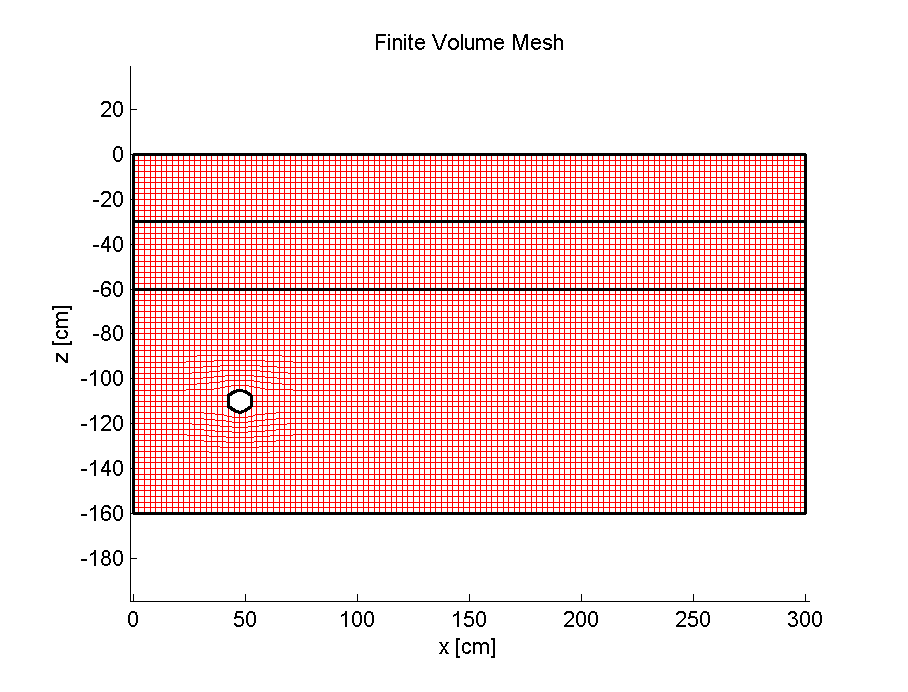
\includegraphics[width=\hsize]{grid_trapz.eps}
\caption{Example of grid consisting of trapezoids.}
\label{fig:grid_trapz}
\end{figure}

\begin{figure}[h]
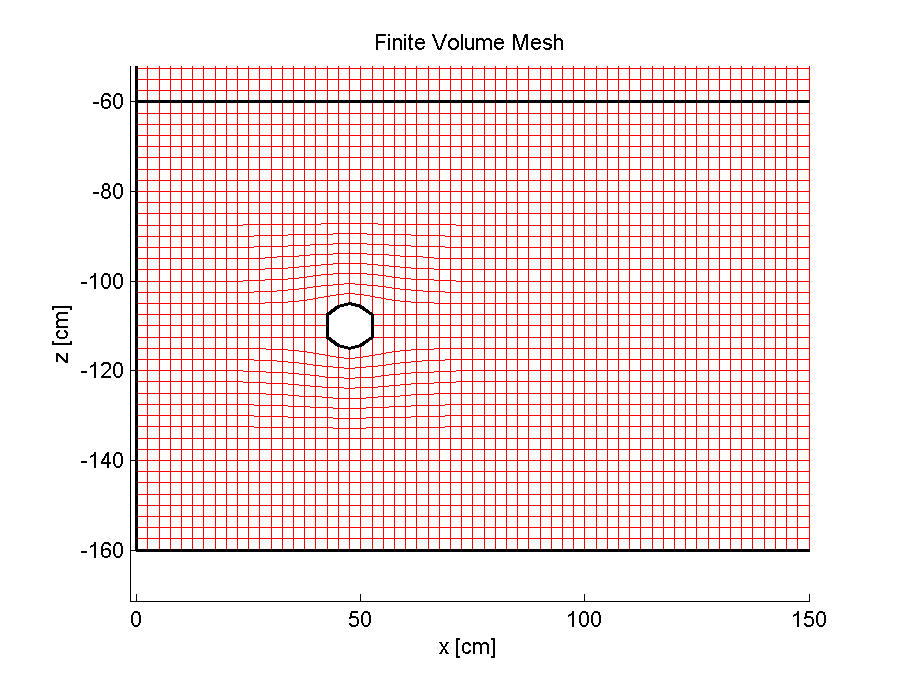
\includegraphics[width=\hsize]{grid_trapz_part.eps}
\caption{Close picture of grid near the drain pipe.}
\label{fig:grid_trapz_part}
\end{figure}


The quadrilateral (rectangular or trapezoid) cells are denoted $Q_i$
where $i=1,2,\cdots, N$. $|Q_i|$ denotes the area of $Q_i$, and
$\partial Q_i$ is the boundary of $Q_i$ i.e. the edges (or faces) of
$Q_i$. All internal edges $e_{ij}$ are labeled by indices, $i$ and
$j$ of the adjacent cells that shares face. The grid is constructed
such that only whole faces are shared ($e_{ij}=Q_i \cap Q_j$). The
length of $e_{ij}$ is $|e_{ij}|$ and the unit normal vector pointing
from $Q_i $into $Q_j$ and orthogonal to $e_{ij}$ is denoted
$\bar{\mathbf{n}}_{ij}$.


$\sigma_i$ contains cell indices of cells sharing faces with cell
$i$. $\sigma_i'$ contain indices of cell faces of cell $i$ which are
placed on $\partial \Omega$, i.e. it is not shared with another
cell.  $\sigma_i'$ is divided into two subsets, $\sigma_{i}'^{D}$
and $\sigma_{i}'^{N}$ of boundary cell faces with a Dirichlet and
Neumann boundary condition, respectively.



\subsection{Cell mass-balances}


Richards equation is integrated over control volume (here a cell),
$Q_i$. By applying the divergence theorem by Green-Gauss, we
obtain
\begin{equation}
\int_{Q_i} \frac{\partial \theta}{\partial t} d \Omega =
\int_{\partial Q_i} \left(\mathbf{K}(\psi)\nabla (\psi + z)
\right)\cdot \mathbf{\bar{n}} dl - \int_{Q_i} \Gamma d\Omega
\label{eq:integratet}
\end{equation}

where $\mathbf{\bar{n}}$ is the outwarded unit normal and $\partial
Q_i$ the boundary of $Q_i$. The cell averages of $\theta$ and $\psi$
are denoted  $\theta_i$ and $\psi_i$. $\theta_i$ and $\psi_i$, $i=1,
2, \cdots N$ where $N$ is the number of cells that are collected in
the vectors $\boldsymbol{\theta}$ and $\boldsymbol{\psi}$.
Discretization  of equation \ref{eq:integratet} based on a grid
consisting of quadrilaterals yield

\begin{equation}
|Q_{i}|\frac{d \theta_i}{dt} = \sum_{j \in \sigma_i} D_{ij}(\boldsymbol{\psi})
 + \sum_{j \in \sigma_i} G_{ij}(\boldsymbol{\psi})
 + \sum_{j' \in \sigma_{i}'} B_{ij'}(\boldsymbol{\psi})
 - S_{i}(\boldsymbol{\psi})
\label{eq:discretised}
\end{equation}

where:

\begin{itemize}
\item $D_{ij}(\boldsymbol{\psi})$ describe the diffusive transport
between internal borders \item $G_{ij}(\boldsymbol{\psi})$
describe the gravitational transport between internal boundaries
\item $B_{ij'}(\boldsymbol{\psi})$ describe flux for external
boundaries $j'\in \sigma_{i}'$
\item $S_{i}(\boldsymbol{\psi})$ is the integrated sink term (point and area distributed sinks) in the cell. \\
\end{itemize}

The diffusive transport from cell $i$ to cell $j$ can be
calculated as

\begin{equation}
D_{ij}(\boldsymbol{\psi})=|e_{ij}|(\mathbf{K}(\boldsymbol{\psi})\cdot (\nabla \psi)_{ij})\cdot \mathbf{\bar{n}}_{ij}
\label{eq:diffusitive}
\end{equation}

For evaluating equation \ref{eq:diffusitive} it is necessary to
estimate the gradient $(\nabla \psi)_{ij}$. $(\nabla \psi)_{ij}$ is
evaluated by a different method for meshes with rectangular cells
than for the more general and complicated case with meshes
consisting of trapezoid cells. The gravitational transport from cell
$i$ to cell $j$ can be calculated as

\begin{equation}
G_{ij}(\boldsymbol{\psi})=|e_{ij}|(\mathbf{K}(\boldsymbol{\psi})\cdot([0\ 1]^T))\cdot \mathbf{\bar{n}}_{ij}
\label{eq:gravitational}
\end{equation}

The boundary flux term is split into the contribution from
boundaries with Neumann and Dirichlet condition respectively:

\begin{equation}
 \sum_{j' \in \sigma_{i}'} B_{ij'}(\boldsymbol{\psi}) = \sum_{j' \in \sigma_{i}'^N}
 B_{ij'}^{N}(\boldsymbol{\psi}) + \sum_{j' \in \sigma_{i}'^D} B_{ij'}^{D}(\boldsymbol{\psi})
\end{equation}

For the boundaries with Neumann conditions we have

\begin{equation}
B_{ij'}^{N}(\boldsymbol{\psi})= -q_{ij'}|e_{ij'}|
\end{equation}

where $q_{ij'}$ is the size of the Darcy flux, perpendicular to the
cell face and positive for flux out from cell $i$. The easiest way
to implement Dirichlet boundary conditions is simply to force
$\psi_i$ to the value that $\psi$ has on the face with Dirichlet
conditions. Conflicts can arise if cell $i$ has more than one face
with a Dirichlet condition. Instead, the Dirichlet boundary
condition is implemented as if the midpoint of the Dirichlet face
was a neighbor cell. Similar to an interior cell face, a diffusive
and a gravitational contribution can be calculated:

\begin{equation}
B_{ij'}^{D}(\boldsymbol{\psi}) = D_{ij'}^{D}(\boldsymbol{\psi}) +
G_{ij'}^{D}(\boldsymbol{\psi})
\end{equation}

where

\begin{eqnarray}
D_{ij'}^{D}(\boldsymbol{\psi})=|e_{ij'}|(\mathbf{K}(\psi_i)\cdot
(\nabla \psi)_{ij'})\cdot \mathbf{\bar{n}}_{ij'} \\
G_{ij'}^{D}(\boldsymbol{\psi})=|e_{ij'}|(\mathbf{K}(\psi_i)\cdot([0\
1]^T))\cdot \mathbf{\bar{n}}_{ij'}
\end{eqnarray}

where the pressure associated with cell $i$ has been used for
calculating the hydraulic conductivity.

The sink term used in equation \ref{eq:continuity} can be divided
into two parts

\begin{equation}
\Gamma=\Gamma_A+\Gamma_p \delta(x_p-x)\delta(z_p-z)
\end{equation}

where $\Gamma_A$ is the contribution from a area distributed sink
and $\Gamma_P$ is the contribution from a point sink. $(x_p,z_p)$
are the coordinates of the point sink which shall be placed in the
interior of a cell(not on the cell faces). $\delta$ is the Dirac
delta function. Thus, the contribution from the sink terms to a cell
yields

\begin{equation}
S_{i}(\boldsymbol{\psi}) = \Gamma_A |Q_i| + \Gamma_P
\end{equation}

Area distributed sinks are typically extraction from roots or (in
Daisy2D) water flow between the soil matrix and macro pore domain.
The point sinks can be tile drains or drip irrigation systems (point
sources). Both $\Gamma_A$ and $\Gamma_P$ can be dependent on the
solution ($\psi$).





\subsection{Rectangular cells}

For the situation with a mesh consisting of rectangular cells, only
matrix pressure in the four neighbor cells (see figure
\ref{fig:meshrect_nswe}) are applied for calculating the fluxes
through the faces of the cell (five point stencil). In the present
section we will only evaluate the gradient for the "eastern" cell
face of cell $i$. The theory can easily be applied for the 3
remaining directions.

\begin{figure}[h]
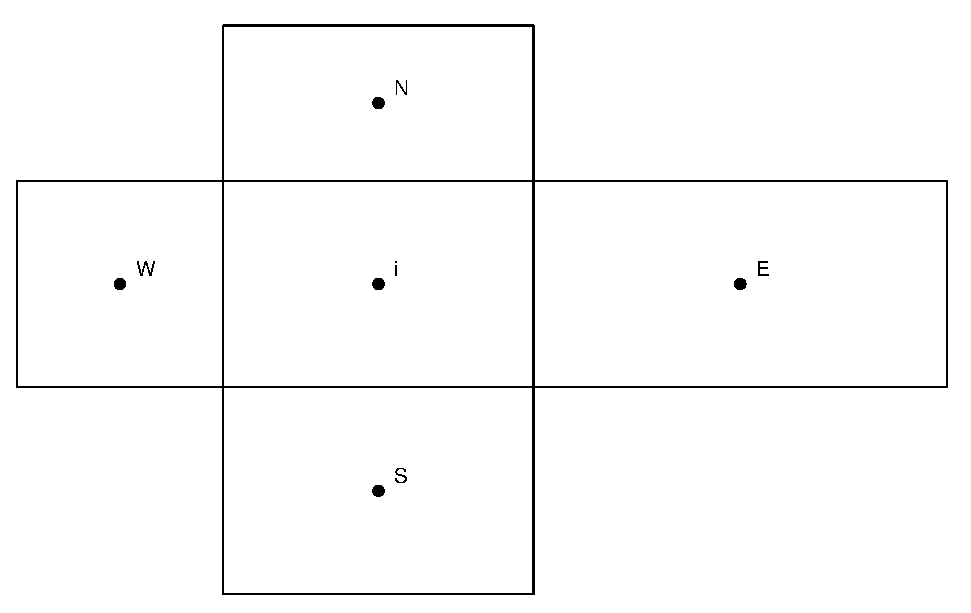
\includegraphics[width=\hsize]{meshrect_nswe.eps}
\caption{Cell $i$ and the neighbor cells it share faces with.}
\label{fig:meshrect_nswe}
\end{figure}

The distances necessary for evaluating the flux from a cell to the
cell placed east of the cell are shown in figure
\ref{fig:meshrect_gradient}.

\begin{figure}
\includegraphics[width=\hsize]{meshrect_gradient.eps}
\caption{Distances used for calculation of flux between cell $i$
and its "eastern" neighbor.} \label{fig:meshrect_gradient}
\end{figure}

The value of $\psi$ in the midpoint of the eastern cell ($\psi_E$)
can be expressed by a Taylor expansion of the value of $\psi$ at
the midpoint of the cell face:

\begin{equation}
\psi_E = \psi(x+\delta x^+)=\sum_{k=0}^{m}  \frac{1}{k!} \left(\frac{d^k \psi}{dx^k}\right)_f (\delta x^+)^k  + R^+
\end{equation}

where $m$ is the order of the Taylor expansion and $R^+$ is the
Lagrange remainder. Similar can $\psi_i$ be computed

\begin{equation}
\psi_i = \psi(x-\delta x^-)=\sum_{k=0}^{m}  \frac{1}{k!} \left(\frac{d^k \psi}{dx^k}\right)_f (-\delta x^-)^k  + R^-
\end{equation}

It can be assumed that $R^+ - (-1)^{m+1}R^- \approx 0$. Thus if a
Taylor expansion of first order ($m=1$) is chosen we get

\begin{equation}
\left( \frac{d \psi}{dx} \right)_f (\delta x^+ +\delta x^-)\approx \psi_E-\psi_i
\end{equation}

If a higher order Taylor expansion is chosen we get

\begin{equation}
\left( \frac{d \psi}{dx} \right)_f (\delta x^+ +\delta x^-)\approx \psi_E-\psi_i - \epsilon_{Ei}
\end{equation}

where the correction term can be calculated as

\begin{equation}
\epsilon_{Ei} \approx \sum_{k=2}^{m}  \frac{1}{k!} \left(\frac{d^k
\psi}{dx^k}\right)_f \left[ (\delta x^+)^k - (-\delta x^-)^k \right]
\end{equation}

It can be seen that a second order precision is obtained with
$m=1$ and $\delta x^+=\delta x^-$. $m=1$ is chosen for the
relative simple model for rectangular cells.



%\begin{equation}
%\sum_{j \in \sigma_i} D_{ij}(\boldsymbol{\psi})=
%\end{equation}


%\begin{equation}
%\sum_{j \in \sigma_i} D_{ij}(\boldsymbol{\psi})=
%\end{equation}


The width and height of cell $i$ are denoted $(\Delta x)_i$ and
$(\Delta z)_i$ respectively, thus $\delta x^{-}= \frac{(\Delta
x)_i}{2}$, $\delta x^{+}= \frac{(\Delta x)_E}{2}$ and
$|e_{iE}|=(\Delta z)_i= (\Delta z)_E$. The outwarded unit normal,
 $\mathbf{\bar{n}}_{iE}=[1\ 0]^T$. By applying equation \ref{eq:diffusitive},
 the diffusive transport through the cell eastern face is:

\begin{equation}
D_{iE}(\boldsymbol{\psi})=(K_{xx})_{iE} \frac{2(\Delta
z)_i}{(\Delta x)_E+(\Delta x)_i}\left(\phi_E-\phi_i \right)
\end{equation}

The gravitational transport from cell $i$ to cell $E$ is:

\begin{equation}
G_{iE}(\boldsymbol{\psi})= 0
\end{equation}

If the eastern cell face of cell $i$ belongs to the boundary of
$\Omega$ (no eastern neighbor), $B_{iE'}$ shall be calculated. If
the cell face has a Neumann boundary condition we have

\begin{equation}
B_{iE'}^N(\boldsymbol{\psi}) = -q_{iE'} (\Delta z)_i
\end{equation}


where $q_{iE'}$ is the magnitude of the flux transported out from
through the cell face. If the cell face have a Dirichlet boundary
condition:

\begin{equation}
D_{iE'}^{D}(\boldsymbol{\psi})=(K_{xx})_{i} \frac{2(\Delta z)_i}
{(\Delta x)_i}\left(\psi_{E'}-\psi_{i} \right)
\end{equation}

where $\psi_{E'}$ is the value of $\psi$ in the midpoint on the
eastern cell face of cell $i$. The gravitational part gives:

\begin{equation}
G_{iE'}^D(\boldsymbol{\psi})= 0
\end{equation}







\subsection{Trapezoid cells - not finished yet!}


\subsubsection{Linear reconstruction}


\begin{equation}
\hat{\psi}(\mathbf{x},t)=\psi_i(t)+\eta_i(\boldsymbol{\psi})\cdot(\mathbf{x}-\mathbf{x}_i), \ \ \mathbf{x} \in Q_i, \ t>0
\end{equation}

Divergence theorem:

Triangles:
\begin{equation}
\overline{\nabla \psi} \approx \sum \psi_j \mathbf{n}_j A_j \approx
\frac{1}{2|T_i|}\mathbf{R}\left[\psi_{\alpha}(\mathbf{x}_{\beta}-\mathbf{x}_{\gamma})
+\psi_{\beta}(\mathbf{x}_{\gamma}-\mathbf{x}_{\alpha})
+\psi_{\gamma}(\mathbf{x}_{\alpha}-\mathbf{x}_{\beta})\right]
\end{equation}

Quadrilaterals:
\begin{equation}
\overline{\nabla \psi} \approx \sum \psi_j \mathbf{n}_j A_j \approx
\frac{1}{2|Q_i|}\mathbf{R}\left[(\psi_{\alpha}-\psi_{\gamma})(\mathbf{x}_{\beta}-\mathbf{x}_{\delta})
+(\psi_{\beta}-\psi_{\delta})(\mathbf{x}_{\gamma}-\mathbf{x}_{\alpha})\right]
\end{equation}

where

\begin{equation}
\mathbf{R}=\begin{bmatrix} 0 & 1 \\ -1 & 0 \end{bmatrix}
\end{equation}



\subsection{Conductivity at cell faces}


The conductivity at the cell faces between adjacent cells (as used
in equations \ref{eq:diffusitive}) are in Daisy calculated by either
the arithmetic, logarithmic of harmonic mean. Physical arguments
speak for applying the harmonic mean:
\begin{equation}
\frac{1}{K_{ij}} = \frac{1}{2}\left[
\frac{1}{K(\psi_i)}+\frac{1}{K(\psi_j)}\right]
\end{equation}



\subsection{Upper boundary condition}


The upper boundary condition describes how much of the applied water
and surface water that infiltrates into the soil. For instance if
the rate of the applied water exceeds the amount of water that can
infiltrate into the soil, (the infiltrability) water is stored on
the surface.

In the start of each of the iterations, within the time step, the
infiltrability is calculated using Darcy's law (based on the
pressure at surface in the last time step and the pressure in the
surface cell.) If the amount of available water (surface water +
applied water in the current time step) exceeds the amount of water
that can infiltrate into the soil as calculated with the
infiltrability, a Dirichlet (pressure) boundary condition is
applied. If the amount of water which can infiltrate into the soil,
as calculated with the infiltrability exceeds the amount of
available water then a Neumann (flux) boundary condition is applied.
The upper boundary can at a given time consists of parts with
Dirichlet and parts with Neumann condition.




\subsubsection{Surface flow} %Maybe

In order to take care of the surface water in simulations with a
rectangular soil domain, a surface flow module is developed. It is
possible to choose between some relatively simple models for the
surface water distribution. In all the models, surface water below a
certain user defined level (detention storage) representing smaller
ponds, is not moved by surface flow. Common for all the models is
that surface water not are added or removed through the eastern and
western boundaries. The total amount of surface water can only
change by application of water and/or infiltration.

In Daisy2D the surface flow model is executed after each time step.
In a later version more physical based model can be included, for
instance a solver of the Saint-Venant equations.

For slightly monotonically sloping surfaces can the Negative and the
\textit{Positive} models be applied. In the \textit{Negative} model
is the slope of the surface negative, i.e. the water tends to move
from the left to the right. In the \textit{Positive} model is the
slope of the surface positive. For horizontal surfaces can the
\textit{None}, \textit{Compare} and the \textit{0D} model be
applied.




\paragraph{Negative}

The surface water in this model tends to move from the left to the
right. Each iteration starts with the most left cell, then the
second from the left, then the third and so on. For a given cell,
the water level is compared to the cell to the right and if the
water level in the left cell is highest, the water level in the two
cells is equaled and the water is conserved. The only violation to
this rule is that the water in the detention storage not is moved.
The iteration procedure ends when the exchanges of water between
cells are below a certain (very low) level. In Figure
\ref{fig:surface_negative} is the effect of the \textit{Negative}
surface model shown.

\begin{figure}[h]
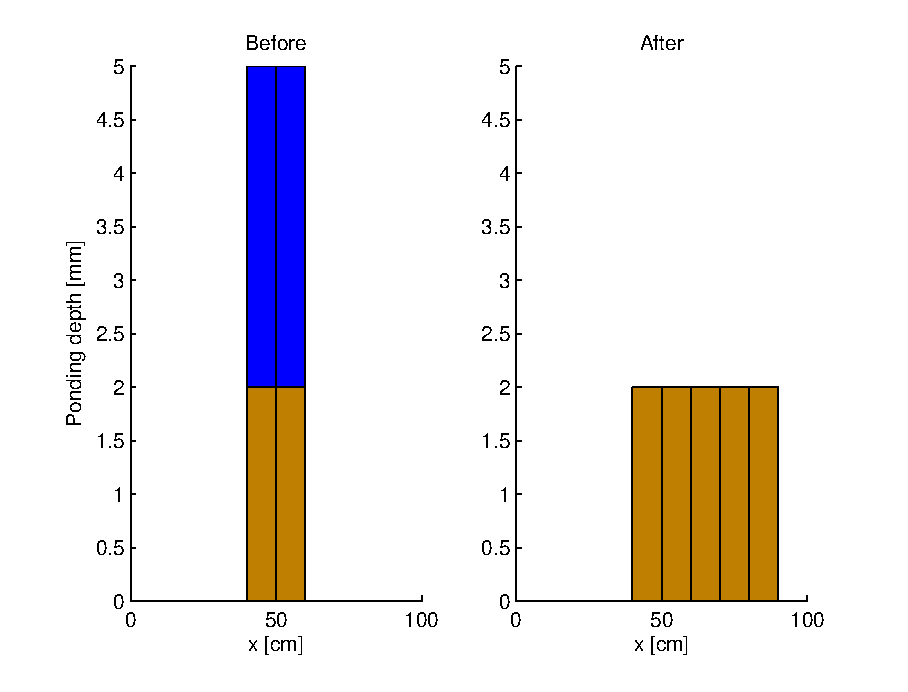
\includegraphics[width=\hsize]{surface_negative.eps}
\caption{Surface water movement with the \textit{Negative} model
with $\Delta x=10$ cm. The left graph shows the surface water
distribution before the redistribution and the right the
distribution after. The brown and blue color represents surface
water below and above the detention storage level, respectively.}
\label{fig:surface_negative}
\end{figure}



\paragraph{Positive}

The model is the reverse of the \textit{Negative model}, i.e. the
water tends to move from the right to the left. In Figure
\ref{fig:surface_positive} is the effect of the \textit{Positive}
surface model shown.

\begin{figure}[h]
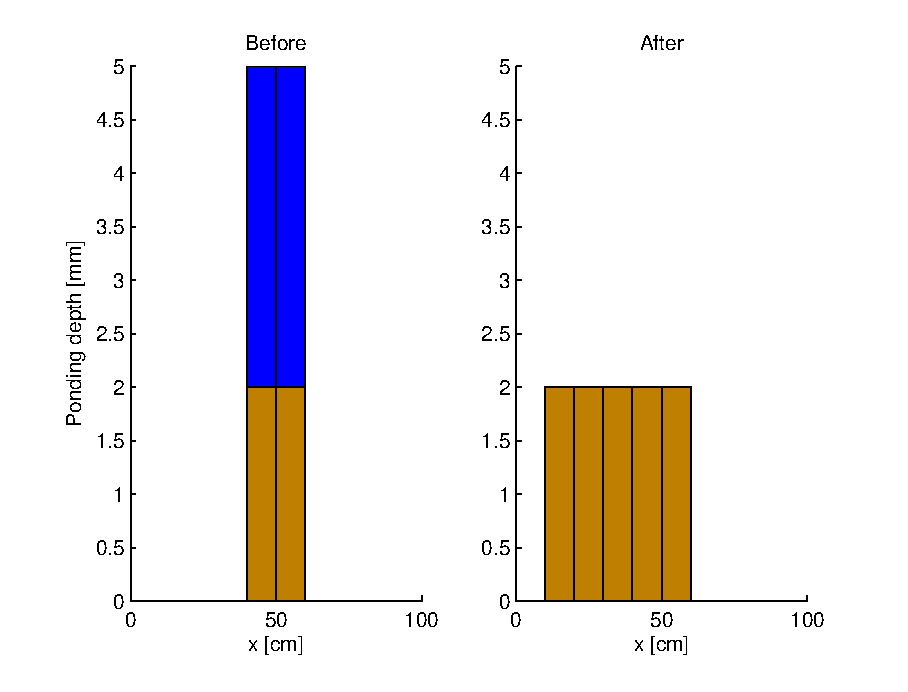
\includegraphics[width=\hsize]{surface_positive.eps}
\caption{Surface water movement with the \textit{Positive} model
with $\Delta x=10$ cm. The left graph shows the surface water
distribution before the redistribution and the right the
distribution after. The brown and blue color represents surface
water below and above the detention storage level, respectively.}
\label{fig:surface_positive}
\end{figure}



\paragraph{None}

In this (none-)model, the surface water is not moved by surface
flow. The model corresponds to the \textit{0D} model with infinitely
large detention storage. In Figure \ref{fig:surface_none} is the
effect of the \textit{None} surface model shown.


\begin{figure}[h]
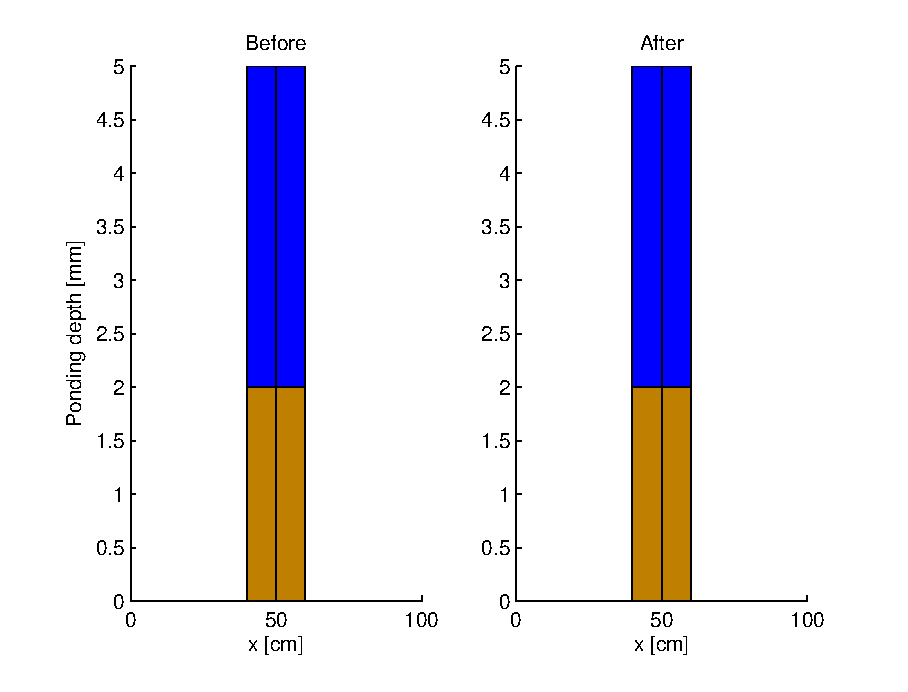
\includegraphics[width=\hsize]{surface_none.eps}
\caption{Surface water movement with the \textit{None} model with
$\Delta x=10$ cm. The left graph shows the surface water
distribution before the redistribution and the right the
distribution after. The brown and blue color represents surface
water below and above the detention storage level, respectively.}
\label{fig:surface_none}
\end{figure}


\paragraph{Compare}

In the \textit{Compare} model, the differences between the surface
water level in neighboring cells are calculated, but only for
neighboring cells where at least one of the cells have a water level
higher than the detention storage. The water in the two cells are
then equaled (with water conservation), but still under the rule
that no water leaves the detention storage. In Figure
\ref{fig:surface_compare} is the effect of the \textit{Compare}
surface model shown.



\begin{figure}[h]
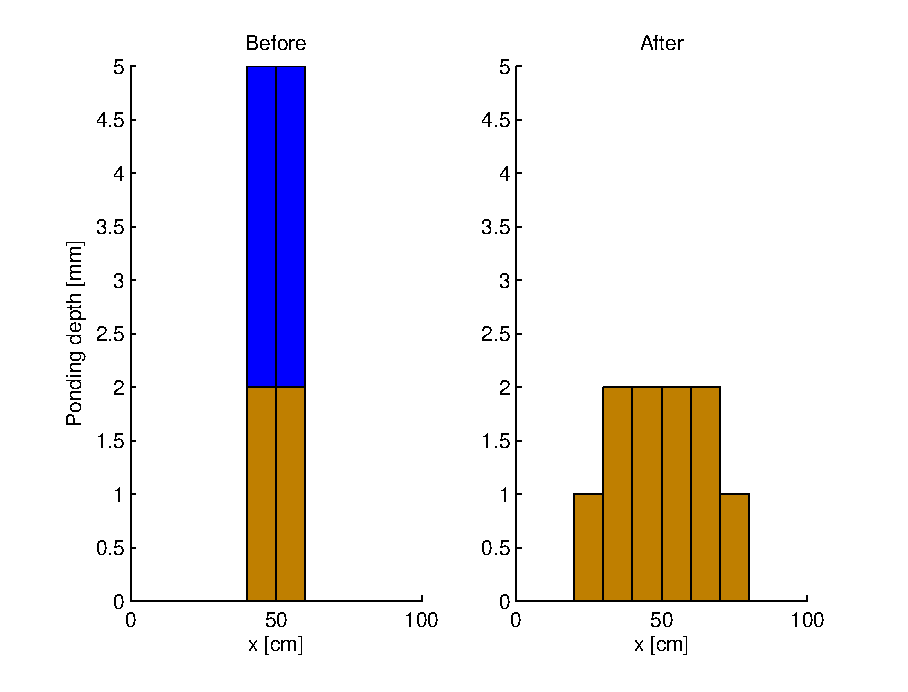
\includegraphics[width=\hsize]{surface_compare.eps}
\caption{Surface water movement with the \textit{Compare} model with
$\Delta x=10$ cm. The left graph shows the surface water
distribution before the redistribution and the right the
distribution after. The brown and blue color represents surface
water below and above the detention storage level, respectively.}
\label{fig:surface_compare}
\end{figure}



\paragraph{0D}

Inside each iteration, all the surface water above the detention
storage level are distributed equally at the surface. In Figure
\ref{fig:surface_0D} is the effect of the \textit{0D} surface model
shown.


\begin{figure}[h]
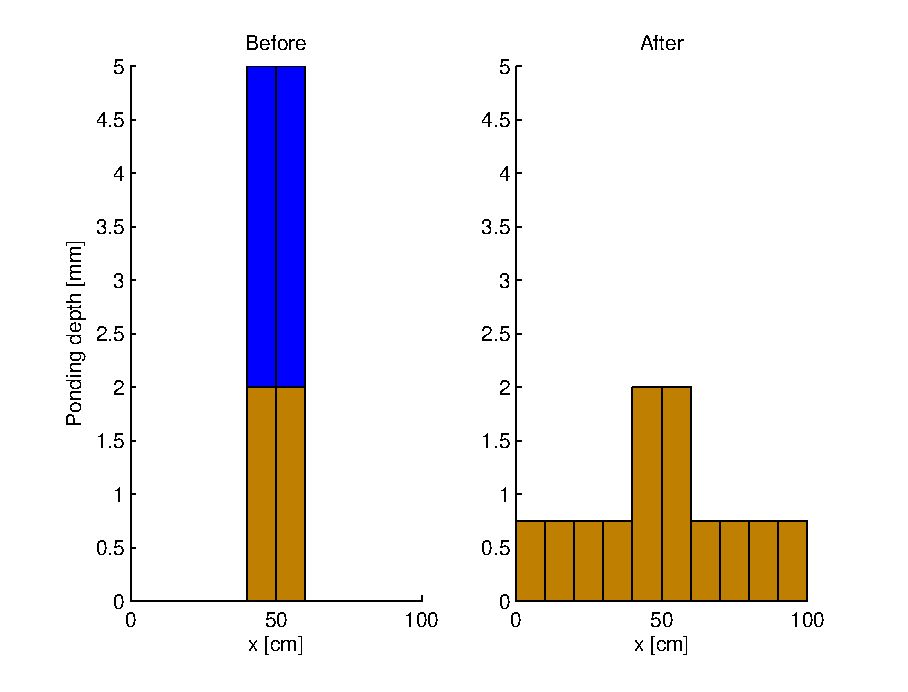
\includegraphics[width=\hsize]{surface_0D.eps}
\caption{Surface water movement with the \textit{OD} model with
$\Delta x=10$ cm. The left graph shows the surface water
distribution before the redistribution and the right the
distribution after. The brown and blue color represents surface
water below and above the detention storage level, respectively.}
\label{fig:surface_0D}
\end{figure}


\subsection{Aquitard boundary condition}

As in the existing 1 dimensional Daisy it is possible to simulate
the existence of an aquitard below the lower boundary of the soil
domain. The aquitard is described by a thickness, a hydraulic
conductivity and the pressure potential in the aquifer just below
the bottom of the aquitard.

In start of the iteration loop, inside each time step, the flow
across the lower boundary is estimated using Darcy�s law where the
pressure in the boundary cells and the properties of the aquitard
are required. The aquitard is then implemented as a Neumann boundary
condition.



\subsection{Tile drains}

It is possible to simulate a (user defined) number of tile drains.
Tile drains removes water when the soil around the drain is
saturated. The actual pressure in a drain pipe depends on position
in the drain system, the hydraulic radius etc, etc. An often applied
simplification codes for variably saturated flow is to regard the
pressure in the drain pipe as atmospheric. When the soil in the
drain point is unsaturated ($\psi<0$) the solution corresponds to
the solution for an undrained soil. If the soil is saturated
($\psi>0$) the drains removes water from the soil matrix hence
$\psi=0$.

In the numerical model, the drain pipe is described as a point. The
drain points shall be placed in the interior of a cell and cannot be
placed at cell edges.

For obtaining a numerical stable solution it is in the beginning of
a new iteration in the time step tested if the mean value of the
matrix pressure in the drain cell and its eastern and western
neighbors (if they exists) exceeds 0. If the mean value is positive
the pressure in the drain cell is forced to zero. After each time
step a mass balance for each of the drain cells is made to calculate
the amount of drained water.

Test simulations show that the code both is able to turn on the
drain when the soil is getting wetter and turn of the drain when the
soil is getting drier. Figure \ref{fig:drainaqui} shows the results
from a simulation with an aquitard boundary condition and a drain.
The upper boundary has a no flux condition, thus the only supply of
water is through the aquitard. As it can be observed, the matrix
pressure potential in the drain is 0.



\begin{figure}[h]
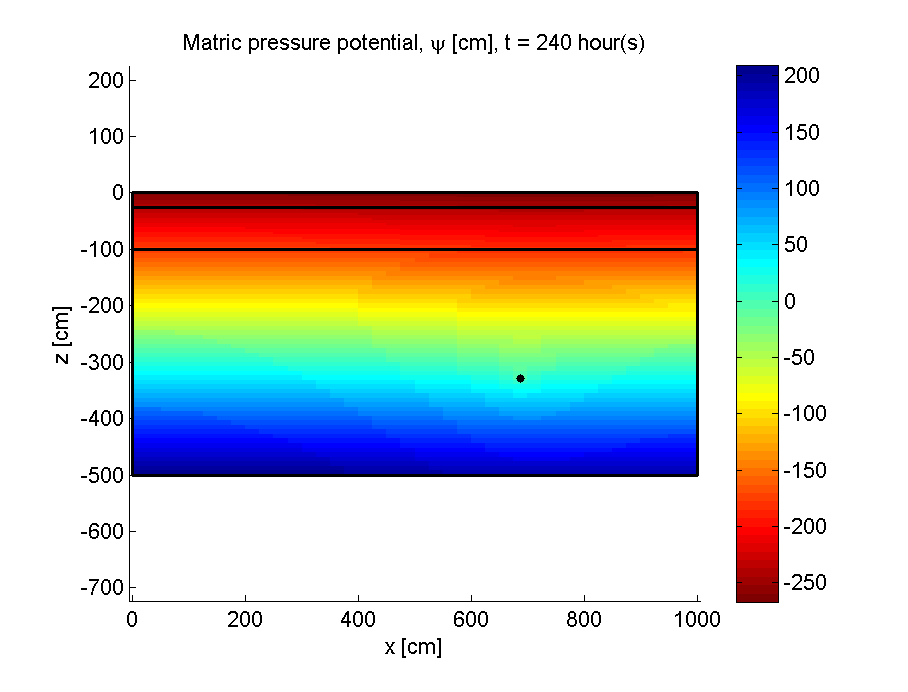
\includegraphics[width=\hsize]{drainaqui.eps}
\caption{Matrix pressure potential in a drained soil. The drain is
indicated with a dot. The lower boundary is formed by an aquitard
condition.}
\label{fig:draintest}
\end{figure}



\subsection{Drip irrigation}



\subsection{Iteration scheme}


Equation \ref{eq:discretised} describes how the matrix pressure
potential in a given cell depends on the matrix pressure potential
in the neighboring cells. By assembling equation
\ref{eq:discretised} for $i=1,\,2\,\cdots N$, the problem can be
written as a ordinary differential equation (ODE) on the form:

\begin{equation}
\mathbf{Q}\frac{d\boldsymbol{\theta}}{dt}=\mathbf{E}(\boldsymbol{\psi})\boldsymbol{\psi}+\mathbf{F}(\boldsymbol{\psi})
\end{equation}

where $\mathbf{Q}$ is a diagonal matrix with $Q(i,i)=|Q_i|$ and
$\theta=\theta(\psi)$.
$\mathbf{E}(\boldsymbol{\psi})\boldsymbol{\psi}$ is the assembly of
$D_{ij}$ and $D_{ij'}^{D}$ and $G_{ij}$, $G_{ij'}^D$, $B_{ij'}^{N}$
and $S_i$ are assembled in $\mathbf{F}(\boldsymbol{\psi})$. The
equation is solved in the time domain using the backward Euler
method:

\begin{equation}
\mathbf{Q}\frac{\boldsymbol{\theta}^{n+1,m+1}-\boldsymbol{\theta}^{n}}{\Delta t}
=\mathbf{E}(\boldsymbol{\psi}^{n+1,m})\boldsymbol{\psi}^{n+1,m}+\mathbf{F}(\boldsymbol{\psi}^{n+1,m})
\end{equation}


In order to get rid of $\theta$ at iteration step $m+1$, the mixed
formulation by \citet{Celia} is applied. In the mixed formulation,
the water content at time step $n+1$ and iteration step $m+1$ is
approximated by a Taylor expansion:

\begin{equation}\begin{split}
\theta^{n+1,m+1}&=\theta^{n+1,m}
+\frac{d\theta}{d\psi}\mid^{n+1,m}(\psi^{n+1,m+1}-\psi^{n+1,m})\\
&=\theta^{n+1,m} +C^{n+1,m}(\psi^{n+1,m+1}-\psi^{n+1,m})
\label{eq:taylor}
\end{split}\end{equation}

where $C=\partial \theta/\partial \psi$ is the specific water
capacity function. The time derivative of $\theta$ can then be
approximated as:

\begin{equation}\begin{split}
\frac{\partial \theta}{\partial t}&\approx
\frac{\theta^{n+1,m+1}-\theta_{n}}{\Delta
  t}=\frac{\theta^{n+1,m+1}-\theta^{n+1,m}}{\Delta
  t}+\frac{\theta^{n+1,m}-\theta_{n}}{\Delta t}\\ & \approx C^{n+1,m}
\frac{\psi^{n+1,m+1}-\psi^{n+1,m}}{\Delta
  t}+\frac{\theta^{n+1,m}-\theta^{n}}{\Delta t}
\end{split}\end{equation}

Thus, the iterative scheme is

\begin{eqnarray}
\left( \frac{1}{\Delta t} \mathbf{QC}(\boldsymbol{\psi}^{n+1,m})-\mathbf{E}(\boldsymbol{\psi}^{n+1,m}) \right)
\boldsymbol{\psi}^{n+1,m+1} = && \nonumber \\
\mathbf{F}(\boldsymbol{\psi}^{n+1,m}) + \frac{1}{\Delta t} \mathbf{QC}(\boldsymbol{\psi}^{n+1,m}) \boldsymbol{\psi}^{n+1,m}
+\frac{1}{\Delta t} \mathbf{Q}\left( \boldsymbol{\theta}^{n}-\boldsymbol{\theta}^{n+1,m} \right)
\label{eq:matrix}
\end{eqnarray}


where $\mathbf{C}$ is a diagonal matrix with $C(i,i)=C_i$. \\
\\
In the MATLAB-prototype it is possible to choose simulations with a
constantly or dynamically size of the time steps, $\Delta t$. For
the last choice, the size of $\Delta t$ depends on how difficult it
is to obtain a solution. A procedure based on same principles is
described in detail in \citet{Mollerupphd}. In Daisy2D the current
Daisy method will be applied.


\subsection{Matrix solution technique}


In the prototype, for solving the large matrix system of the type
$\mathbf{Ax}=\mathbf{b}$ (see equation \ref{eq:matrix}), the MATLAB
backslash operator (also called leftdivision) is used. For
description of the applied sparse matrix solver is refereed to
\citet{Mollerupphd}.


\subsection{Hydraulic properties}

In the Daisy2D it shall be possible to choose between the existing
models for the soil hydraulic properties in Daisy. In the prototype,
the retention characteristics are described with the model by
\citet{vanGenuchten}:
%%% with moustages %%%
\begin{equation}
\theta=\begin{cases} \theta_{r} +
\frac{\theta_s-\theta_r}{[1+|\alpha \psi|^n]^m} & \text{for
  $\psi<0$}\\
\theta_{s} &\text{for $\psi \geq 0 $} \end{cases}
\end{equation}
%%%%%%%%%%%%%%%%%%%%%
%%% without moustages %%%
%\begin{eqnarray}
% \theta= \theta_{r} + \frac{\theta_s-\theta_r}{[1+|\alpha
%\psi|^n]^m} && \text{for
%  $\psi<0$} \nonumber \\
% \theta= \theta_{s} && \text{for $\psi \geq 0 $}
%\end{eqnarray}
%%%%%%%%%%%%%%%%%%%%%%




where $\alpha$, $n$ and $m$ are empirical parameters, $\theta_s$ and
$\theta_r$ are the saturated and the residual water content,
respectively. By combination with the hydraulic conductivity model
by \citet{Mualem} and choosing $m=1-1/n$, the hydraulic conductivity
can be calculated as
\begin{equation}
K=K_sS_{e}^{1/2}[1-(1-S_{e}^{1/m})^m]^2
\end{equation}
where $K_s$ is the hydraulic conductivity at saturation and $S_e$
is the effective saturation defined as
\begin{equation}
S_e=\frac{\theta-\theta_r}{\theta_s-\theta_r}
\end{equation}
The retention model by van Genuchten has been adapted to a large
class of soils.


\subsection{Ridge - not for first report!}

For describing the geometry and producing the finite element mesh
is the general FEM-code, \citet{FEMLAB} used. In the actual case
the two-dimensional geometry described using a so called geometry
m-file. Of geometrical reasons only the half of a ridge is
described. The soil profile is divided into 7 strata or subdomains
with different soil properties which are described elsewhere in
the paper. The ridge with the different subdomains is plotted in
figure XXX. The ridge height can be described with a sine
function:
\begin{equation}
f(x)=A \left[ 1+sin\left(-\frac{\pi}{2}+2\frac{\pi x}{W}\right)
\right], \ \ \ 0 \leq x \leq W/2
\end{equation}
where $W$ is the width of the ridge and $A$ is the amplitude of the
sine wave which is the same as half of the ridge height. The curve
only describes half a ridge that will be used for the modeling.


\section{Verification}

The FVM-code is verified by comparing solutions obtained by FVM with
quasi-analytical solutions for one-dimensional infiltration by
Philip.


\subsection{Infiltration Model of Philip}


\citet{Philip} showed that the infiltration depth as function of
time and saturation can be written as a power series in
$t^{\frac{1}{2}}$. The coefficients are then functions of soil water
content, $\theta$. From the expression for the infiltration depth,
as function of water content and time, it is relatively easy to
derive that the cumulative infiltration, also can be written as a
power series in $t^{\frac{1}{2}}$. The assumptions for the theory,
is a 1-dimensional vertical flow into a homogenous soil
semi-infinite soil column, initially with uniform water content. The
cumulative infiltration is expressed as

\begin{equation}
I=\sum_{n=1}^{+\infty}A_n t^{\frac{n}{2}}
\label{eq:Philip}
\end{equation}

where $A_1=S$ is the often refereed sorptivity as defined in
\citet{PhilipAdv}. The coefficients are found by solving a set of
successive integro-differential equations. One drawback of the
power series theory is that the theory only describes the
infiltration process well for short to intermediate times. The
power series is "practical convergent" for $t<t_{\text{grav}}$.
Where $t_{\text{grav}}$ is the characteristic time of the
infiltration process

\begin{equation}
t_{\text{grav}}=\left(\frac{S}{K_0-K_i} \right)^2
\label{eq:tgrav}
\end{equation}

where $K_i=K(\theta_i)$ and $K_0=K(\theta_0)$ is the hydraulic
conductivity corresponding to the initial water content,
$\theta_i$ and the water content at the soil surface, $\theta_0$.
For ponded conditions at the
soil surface we have $K_0=K_s$. \\
\\
The soil parametrization, which is applied for the test simulations,
is the G.E. silt loam \citep{vanGenuchten} where $K_s=4.96$ cm/day,
$\theta_s=0.396\ \text{cm}^3/\text{cm}^3$, $\theta_r=0.131\
\text{cm}^3/\text{cm}^3$, $\alpha=0.00423\ \text{cm}^{-1}$ and
$n=2.06$. \\


A constant size of $\Delta t$= 1/60 day has been applied in the FVM
test simulations. For all simulations the initial condition is
$h_i$=-200 cm, corresponding to $\theta_i=0.332\
\text{cm}^3/\text{cm}^3$ is chosen.


\subsubsection{Vertical falling-head infiltration}

Initially, it was shown that the power series solution can be
applied for non-saturated or just saturated conditions at the soil
surface \citep[see][]{PhilipTrans,Philip,PhilipAus}. \citet{Philip6}
later expanded the theory to cover ponding situations with constant
positive pressure at the soil surface. Later it was shown
\citep[][]{Mollerup} that the power series solution also can be
applied for a falling-head condition, where the ponding depth is
dependent on the amount of infiltrated water. The pressure at the
soil surface is then
\begin{equation}
H=H_0-I
\end{equation}
where $H_0$=20 cm is the initial ponding depth.\\
\\
In the FVM simulations, both the vertical and horizontal
discretisation, $\Delta z=\Delta x$ is 1 cm. The lower boundary was
placed at $z=600$ cm with a free drainage (gravity flow) condition.
For the scenario is $t_{\text{grav}}$=3.34 days and the time at
which the pond empties, $t_p=$2.6022 days is computed by applying
the iteration procedure as proposed in \citet{Mollerup}. In
FVM-simulation, the pond empties at approximately $t=$2.5833 days.
I.e. $t_p$ is approximately 0.7\% higher for the power series
solution than for the similar FVM results obtained with a rather
rough discretization in time. Minor errors can be expected in the
power series solution as only the first 4 terms are calculated. For
constant-head simulation the first 6 terms are calculated.
\citet{Philip} found that normally only first two or three terms are
necessary for a for practical use sufficient correct solutions.

In Figure \ref{fig:VerificFH}, the wetting profiles as calculated
by applying FVM and the power series theory are shown. The wetting
profiles are shown for $t=1/5,\, 2/5,\, 3/5,\, 4/5$ and $1\cdot
t_{\text{p}}$. As it can be observed, the solutions are almost
identical except for $t=t_{\text{p}}$ (2.6022 days) where the
effects of the slightly earlier emptying ponded water in the FVM
simulation instantly effects the water content profiles.


\begin{figure}
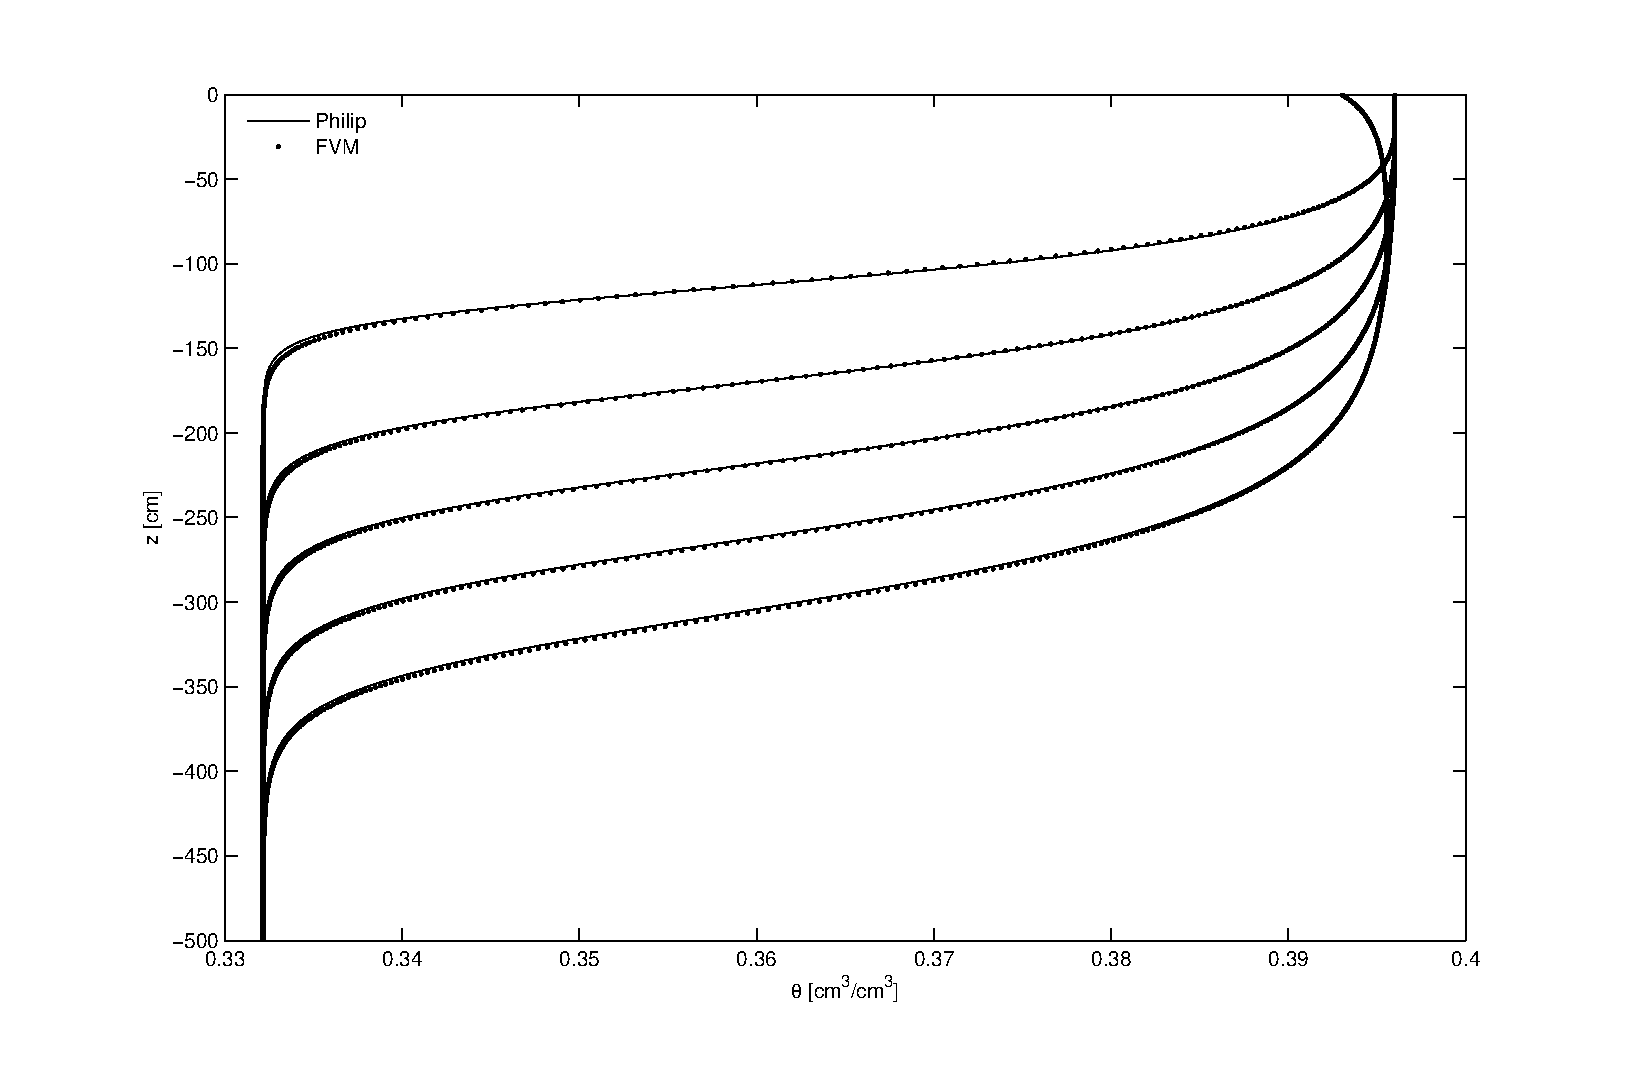
\includegraphics[width=\hsize]{VerificFH.eps}
\caption{Analytical and FVM solution for vertical falling head infiltration. The solution is shown for
$t=1/5,\, 2/5,\, 3/5,\, 4/5$ and $1\cdot t_{\text{p}}$.}
\label{fig:VerificFH}
\end{figure}


\subsubsection{Horizontal constant-head infiltration}

For also insuring that horizontal flows are simulated correctly a
simulation with a horizontal oriented column is made. For the FVM
simulation, the column has height of 1 cell and a width of 800 cells
with $\Delta x=\Delta z=$1 cm. The left boundary condition is $H=$20
cm and the initial condition is $h_n=$-200 cm. Vertical
constant-head infiltration can analytically be calculated as:

\begin{equation}
I=A_1 \sqrt(t)
\label{eq:horizontal}
\end{equation}

where $A_1$ is identical to the $A_1$ calculated for vertical
infiltration with constant-head (and falling-head) conditions.
Contrary to vertical infiltration, equation \ref{eq:horizontal} is
applicable also for longer periods. Figure \ref{fig:VerificHor}
shows the water content profiles at $t=1/5,\, 2/5,\, 3/5,\, 4/5$ and
$1\cdot t_{\text{grav}}$. as calculated with FVM and the power
series theory. As it can be seen are the solutions almost identical.

\begin{figure}
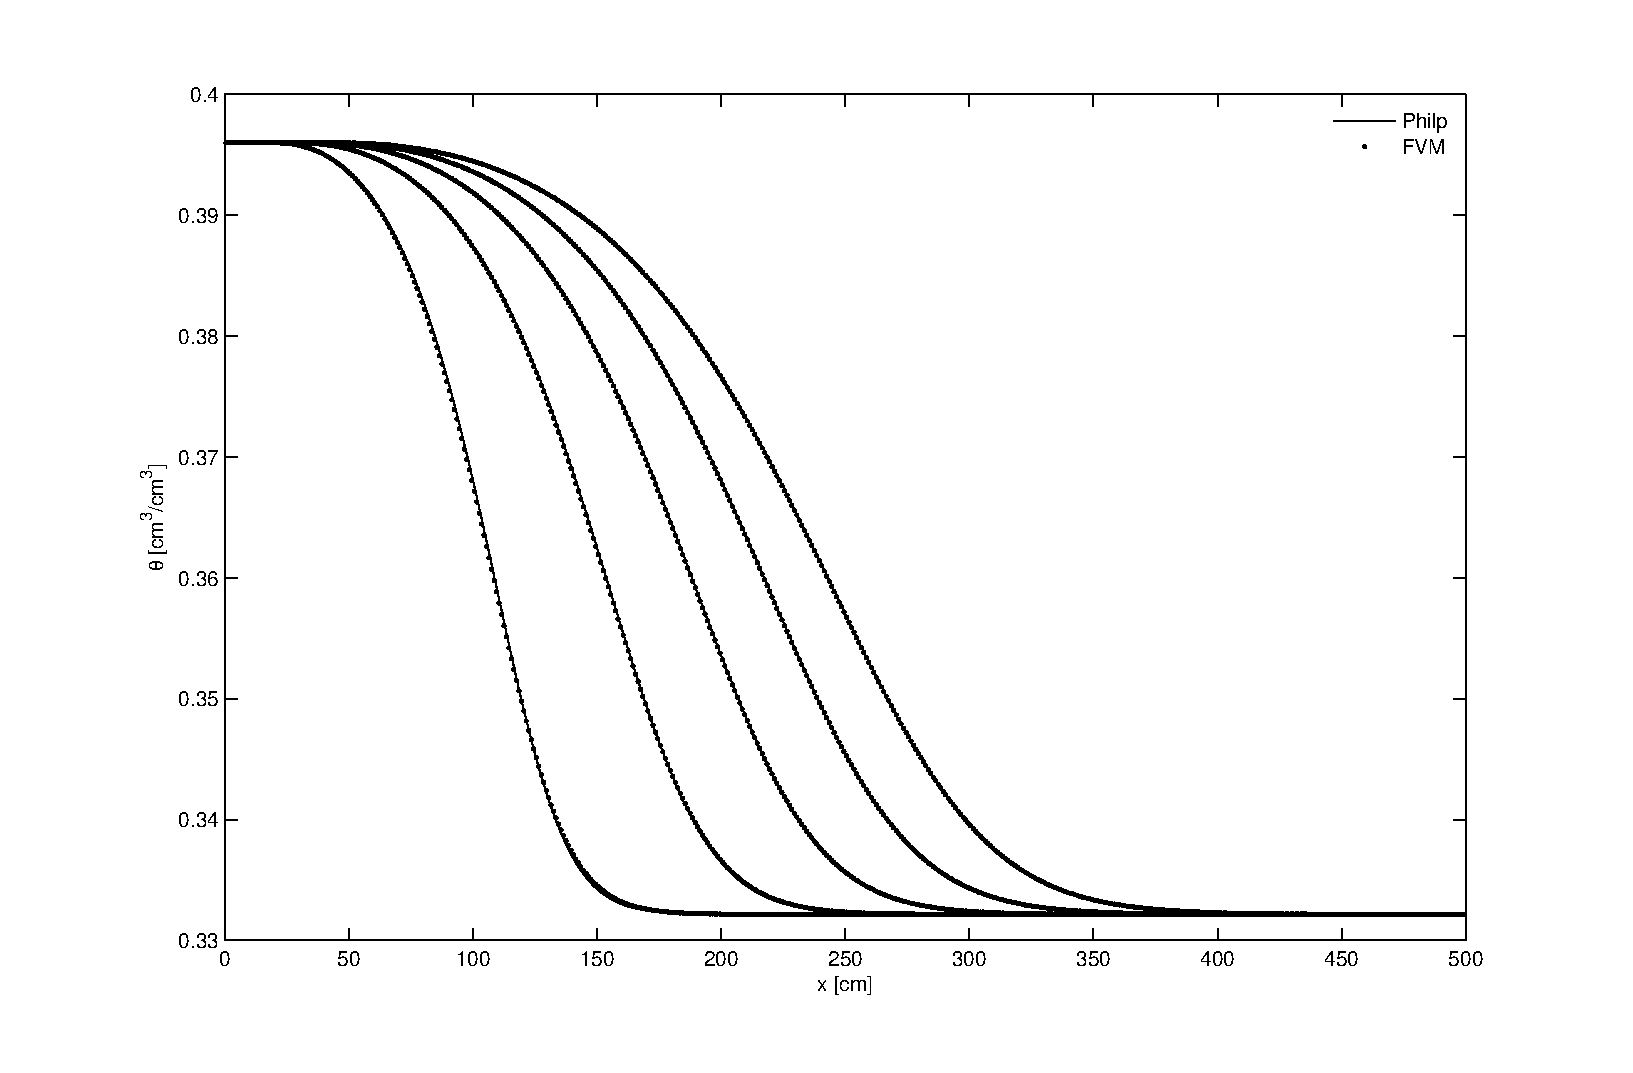
\includegraphics[width=\hsize]{VerificHor.eps}
\caption{Analytical and FVM solution for horizontal infiltration. The solution is shown for
$t=1/5,\, 2/5,\, 3/5,\, 4/5$ and $1\cdot t_{\text{grav}}$.}
\label{fig:VerificHor}
\end{figure}


\subsection{Vertical constant-head infiltration in a wide column}

Until now all the verification simulations are made for a grid
consisting of only 1 cell in the direction perpendicular to the flow
direction. Also the size of the cells was equal. In the wide column
experiment the cell height varies with the depth. The soil column
consists of 3 horizons (A, B and C). The A-horizon is 25 cm depth
with $\Delta z=$1 cm, the B-horizon is 75 cm depth with $\Delta z=$3
cm, and the C-horizon is 400 cm depth with $\Delta z=$8 cm. The soil
column have a width of 200 cm with $\Delta x=$20 cm. Figure
\ref{fig:Mesh} shows the mesh and figure \ref{fig:MeshPart} shows a
upper part of the mesh.


\begin{figure}
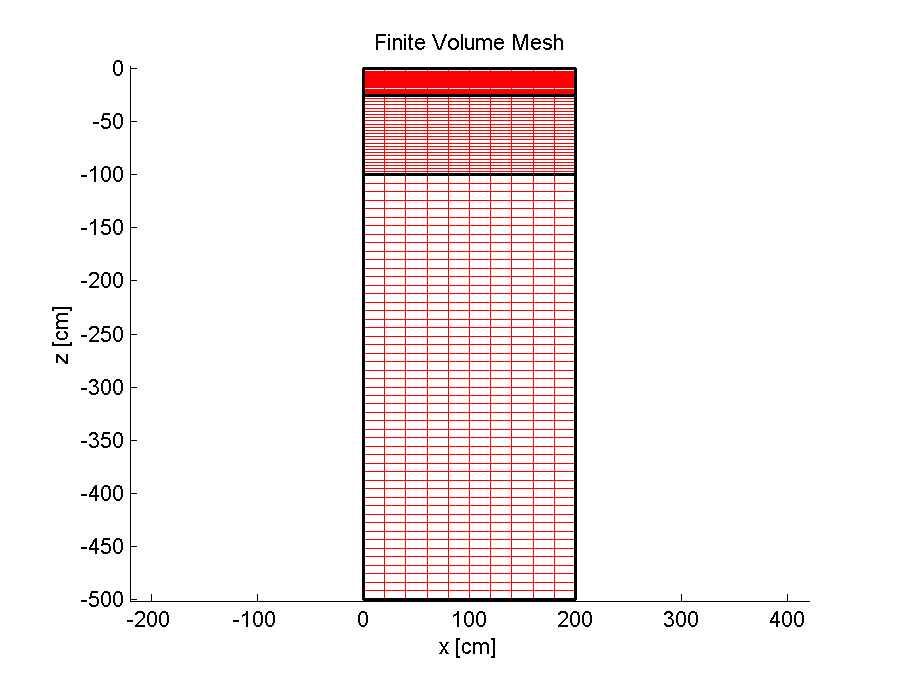
\includegraphics[width=\hsize]{Mesh.eps}
\caption{Mesh for the wide column simulation.}
 \label{fig:Mesh}
\end{figure}


\begin{figure}
\begin{center}
\includegraphics[width=\hsize]{MeshPart.eps}
\caption{Upper left part of mesh used for the wide column
simulation.}
 \label{fig:MeshPart}
\end{center}
\end{figure}


In the simulation is the ponding depth constantly $H=20$ cm. Figure
\ref{fig:VerificRect} shows the water content after 1 day. As it can
be observed, the water do not vary with the x-coordinate for a given
depth, i.e. there is no indication of unintended exchange of water
between internal vertical cell boundaries.


\begin{figure}
%\includegraphics[width=\hsize]{lalala.eps}
%\includegraphics{lalala.eps}
\includegraphics[width=\hsize]{watercontent24h.eps}
\caption{Water distribution after 1 day in the wide column
simulation.}
 \label{fig:VerificRect}
\end{figure}


Also here (not shown) comparisons with a power series solution
shown fine agreement


\subsection{Other simulations}

Also a simulation with a Neumann (flux) condition at the upper
boundary and a simulation with a non-zero sink term have been
conducted. The simulations showed mass-balances with negligible
errors.



%\section{Referencer}
%
%
%Liste med referencer:\\
%\\
%
%\begin{itemize}
%\item \citep{Mollerupphd}\\
%\item \cite{Philip} \\
%\item \cite{PhilipTrans,PhilipAus}
%\end{itemize}




% ------------------------------------------------------------------------ %%
%
%  REFERENCE LIST AND TEXT CITATIONS
%
%% ------------------------------------------------------------------------ %%


\bibliographystyle{natbibDK}
\bibliography{MST}


\end{document}
